\documentclass[aspectratio=169]{beamer}

% setup basic metainfo
\title{Balancing Space Complexity and Ambiguity in Superadditive Set Functions}

\usepackage[utf8]{inputenc}
\usepackage{csquotes}
\usepackage{graphicx, xcolor}
\usepackage{mfirstuc}
%\usepackage[defaultmono]{droidmono}
\usepackage{amsmath,amssymb,amsthm,textcomp,thm-restate}
\usepackage{listings}
\usepackage{parskip}
\usepackage{stmaryrd} % lightning symbol n stuff
\usepackage[noend]{algpseudocode}
\usepackage{tikz}
\usepackage{indentfirst}
\usetikzlibrary{positioning}


% handle fonts encoding.
\usepackage[utf8]{inputenc}
\usepackage[T1]{fontenc}

% hyperlinks
\usepackage[capitalize]{cleveref}
\hypersetup{
	colorlinks=false
}

\numberwithin{equation}{section}
\numberwithin{equation}{subsection}
\renewcommand*{\theequation}{%
	\ifnum\value{subsection}=0 %
		\ifnum\value{section}=0 %
		\else\thesection.\fi\else\thesubsection.\fi\arabic{equation}%
}

% small matrix with parenths
\newenvironment{psmallmatrix} {\left(\begin{smallmatrix}} {\end{smallmatrix}\right)}

\algrenewcommand\algorithmicthen{\textbf{:}}
\algrenewcommand\algorithmicdo{\textbf{:}}
\algrenewcommand\algorithmicelse{\textbf{else :}}
\algdef{SN}[SUBALG]{Indent}{EndIndent}{}{}%
\algdef{SN}[SUBALG]{Procedure}{EndProcedure}[2]{\algofont{#1}({#2}):}{}%

% acronyms
%\usepackage[automake]{glossaries-extra}
%\setabbreviationstyle[acronym]{long-short}
%\newacronym{satnarka}{PŠ}{Princip Šatnářky}
%\makeglossaries

% text spread on page
% \usepackage{geometry}
% \geometry{left=25mm,right=25mm,%
% 	bindingoffset=0mm, top=20mm,bottom=20mm}

\def\theorempre{1.7ex plus 1.2ex minus 0.6ex}
\def\theorempost{1.5ex plus 1.2ex minus 0.6ex}

% % custom theorems
% \newtheoremstyle{Sdefi}{\theorempre}{\theorempost}{\normalfont}{0pt}
% {\scshape}{: }{0pt}{{\thmname{#1 }}{\thmnumber{#2}}{\thmnote{ (#3)}}}
% \newtheoremstyle{Sthm}{\theorempre}{\theorempost}{\normalfont}{0pt}
% {\scshape}{: }{0pt}{{\thmname{#1 }}{\thmnumber{#2}}{\thmnote{ (#3)}}}
% \newtheoremstyle{Sex}{\theorempre}{\theorempost}{\normalfont}{0pt}
% {\scshape}{: }{0pt}{{\thmname{#1 }}{\thmnumber{#2}}{\thmnote{ (#3)}}}

\renewcommand{\qedsymbol}{$\blacksquare$}
\def\qed{{\parfillskip=0pt\allowbreak\hfill\nobreak $\blacksquare$\par}}

% code listing settings
\lstset{
	language=Python,
	%basicstyle=\ttfamily\small,
	%backgroundcolor=\color{lightgray},
	aboveskip={1.0\baselineskip},
	belowskip={1.0\baselineskip},
	columns=fixed,
	xleftmargin=2\parindent,
	extendedchars=true,
	breaklines=true,
	tabsize=4,
	prebreak=\raisebox{0ex}[0ex][0ex]{\ensuremath{\hookleftarrow}},
	showtabs=false,
	showspaces=false,
	showstringspaces=false,
	%keywordstyle=\color{blue},
	%commentstyle=\color{teal},
	%stringstyle=\color{teal},
	numbers=left,
	captionpos=b
}

% misc
\def\restrict#1#2{#1\!\restriction\!#2}
\def\doubleunderline#1{\underline{\underline{#1}}}
\def\rand#1{\text{#1}}
\def\randvec#1{\textbf{#1}}

\def\suchthat{;\,}
\def\given{;}

\def\pot#1{\fce{\mathcal{P}}{#1}}
\def\potfin#1{\left[ #1 \right]^{<\omega}}
\def\xor{\mathbin{\oplus}}
\def\divides{\mathbin{\backslash}}

% functions with auto parenths
\def\bfce#1#2{#1\!\bigl(#2\bigr)}
\def\fce#1#2{#1\!\left(#2\right)}
\def\fceb#1#2{#1\!\left[ #2 \right]}
\def\fcec#1#2{#1\{#2\}}
\def\fces#1#2{#1\!\left< #2 \right>}

\def\algofont{\textsc}
\def\algref#1{\algofont{\nameref{#1}}}
\def\algorithm#1#2{\fce{\algofont{#1}}{#2}}
\newenvironment{algor}[3]{\begin{minipage}{\textwidth}\begin{algo}[#1]\ \\ \AlgIn #2\\\AlgOut #3 \begin{algorithmic}[1]}{\end{algorithmic}\end{algo}\end{minipage}}

\def\set#1{\left\{#1\right\}}
\def\arr#1{\left[#1\right]}

\DeclareMathOperator{\conv}{conv}
\DeclareMathOperator{\cov}{cov}
\DeclareMathOperator{\var}{var}
\DeclareMathOperator{\fin}{Fin}
\DeclareMathOperator{\poly}{poly}
\DeclareMathOperator{\dlog}{dlog}
\DeclareMathOperator{\dom}{dom}
\DeclareMathOperator{\rng}{rng}
\DeclareMathOperator*{\argmin}{arg\,min}
\DeclareMathOperator*{\argmax}{arg\,max}
\DeclareMathOperator{\id}{id}
\DeclareMathOperator{\sgn}{sgn}
\DeclareMathOperator{\adj}{adj}
\DeclareMathOperator{\Ker}{Ker}
\DeclareMathOperator{\rank}{rank}
\DeclareMathOperator{\trace}{trace}
\DeclareMathOperator*{\mini}{mini}
\DeclareMathOperator*{\maxi}{maxi}
\DeclareMathOperator*{\avg}{avg}

\def\funcs#1#2{^{#1}#2} % množina funkcí z #1 do #2

\def\isomorph{\cong}
\def\dd{\,\text{d}}
\def\compl#1{\overline {#1}}
\def\tuple#1{\left< #1 \right>}

\def\range#1{\left[ #1 \right]}

% vectors
\def\tr{{\!\top\!}}
\def\trans#1{{#1}^{\tr}}
\def\vec{\boldsymbol}
\def\Rmm#1#2{\R^{#1 \times #2}}
\def\Rm#1{\R^{#1}}
\def\ii#1#2{_{#1,#2}}
\def\inv#1{#1^{\inve}}
\def\inve{-1}
\def\I#1{I_{#1}}
\def\zero{\vec{o}}

% probability and random variables
\def\pr#1{\fceb{\Pr}{#1}}
\def\prfa#1#2{\fceb{\Pr_{#1}}{#2}}
\def\prt#1{\fceb{\Pr}{\text{#1}}}
\def\prfat#1#2{\prfa{#1}{\text{#2}}}
\def\vrv{\textbf}
\def\rv{\text}
\DeclareMathOperator*{\E}{\mathbb{E}}

% distributions
\def\Normd{\mathcal{N}}
\def\normd{\fce{\Normd}}
\def\normdf#1#2#3{\normd{#3 \given #1, #2}}
\DeclareMathOperator{\Berd}{Ber}
\def\berd{\fce{\Berd}}
\def\berdf#1#2{\berd{#2 \given #1}}
\DeclareMathOperator{\Poisd}{Pois}
\def\poisd{\fce{\Poisd}}
\def\poisdf#1#2{\poisd{#2 \given #1}}

\def\Rowsp#1{\mathcal{R}\!\left(#1\right)}
\def\Colsp#1{\mathcal{S}\!\left(#1\right)}

\def\norm#1{\left\lVert #1 \right\rVert }
\def\aabsolute#1{\left\lVert #1 \right\rVert }
\def\absolute#1{\left\lvert #1 \right\rvert }
\def\dotpr#1#2{\langle #1 , #2 \rangle}
\def\randin{\in_R}

\def\emod#1{\mathbin{\equiv_{#1}}}
\def\po{\mathbin{\circ}}

\def\disjcup{\mathbin{\dot\cup}}
\def\bigdisjcup{\mathop{\dot\bigcup}}

\def\deltap{\delta^+}
\def\deltam{\delta^-}

\def\deq{\mathbin{:=}}
\def \lHeq{\mathbin{\stackrel{l'H}{=}}}
\def\concat{\cdot}

\def\R{\mathbb{R}}
\def\Q{\mathbb{Q}}
\def\N{\mathbb{N}}
\def\C{\mathbb{C}}
\def\Z{\mathbb{Z}}
\def\K{\mathbb{K}}
\def\P{\mathbb{P}}
\def\V{\mathbb{V}}
\def\F{\mathbb{F}}
\def\ff{\mathcal{F}}
\def\T{\mathbb{T}}
\def\O{\mathcal{O}}
\def\M{\mathcal{M}}
\def\integ#1#2#3#4{\int_{#1}^{#2} #4 \text{d}#3}
\def\iinteg#1#2#3#4{\iint_{#1} #4 \text{d}#2\text{d}#3}

% mohutnost
\def\mohge{\succcurlyeq}
\def\mohgt{\succ}
\def\mohle{\preccurlyeq}
\def\mohlt{\prec}
\def\moheq{\approx}

% implications
\def\implies{\rightarrow}
\def\impliedby{\leftarrow}
\def\Implies{\Longrightarrow}
\def\Impliedby{\Longleftarrow}
\def\iff{\leftrightarrow}
\def\Iff{\Longleftrightarrow}

% complexity classes
\def\problem{\textsc}
\def\problemClass{\textsf}
\def\np{\problemClass{NP}}
\def\p{\problemClass{P}}
\def\conp{\problemClass{coNP}}
\def\fnp{\problemClass{FNP}}

\def\Shapley{\phi}
\newcommand\shapley[1][]{\fce{\Shapley_{#1}}}
\def\k{\mathcal{K}}

% \documentclass [14pt,xcolor=dvipsnames,aspectratio=169]{beamer} 
\usetheme{metropolis}
\setbeamertemplate{caption}{\raggedright\insertcaption\par}
\metroset{block=fill}

\definecolor{mDarkBrown}{RGB}{45, 8, 26}
\definecolor{mDarkTeal}{RGB}{45, 8, 26}
\definecolor{mLightBrown}{RGB}{229, 0, 112}
\definecolor{mLightGreen}{RGB}{229, 0, 112}

\author[1]{Filip \'{U}radn\'{i}k \hfill Supervisor: Mgr. David Sychrovský}
% \institute{Charles University, Prague, Czech Republic}
\date{September 6, 2024}

% english localisation
\usepackage[english]{babel}
% \renewcommand{\lstlistingname}{Code sample}
% \renewcommand{\lstlistlistingname}{List of Code Samples}
% also: defi, thm, algo, glossary

\newtheorem{defi}[equation]{Definition}
\newtheorem{notation}[equation]{Notation}

% \newtheorem{lemma}[equation]{Lemma}
\newtheorem{algo}[equation]{Algorithm}
\newtheorem{obs}[equation]{Observation}
\newtheorem{prop}[equation]{Proposition}
\newtheorem{invar}[equation]{Invariant}
\newtheorem{cor}[equation]{Corollary}

\newtheorem{examp}[equation]{Example}
% \newtheorem{fact}[equation]{Fact}
% \newtheorem{note}[equation]{Note}


\newcommand{\glostitle}{Glossary}


\usepackage[natbib=true,style=authoryear,backend=bibtex,useprefix=true,maxbibnames=4]{biblatex}
\addbibresource{bibliography.bib}
\setbeamertemplate{caption}{\raggedright\insertcaption\par}

\def\blue#1{{\color{blue} #1}}
\def\orange#1{{\color{orange} #1}}
\def\red#1{{\color{red} #1}}
\def\s{\mathcal{S}}

\begin{document}
\maketitle

\begin{frame}{Set Functions}
	\begin{itemize}
		\item<1-> Used in countless fields, including cooperative game theory, combinatorial auctions, matroids.
		\item<2-> Finite \emph{ground set} $ N = \left\{ 1, \ldots, n \right\} $.
		\item<3-> A \emph{(complete) set function} is then any function \[
			f: \pot N \to \R.
		\]
	\end{itemize}
\end{frame}

\begin{frame}{What Is Wrong?}
	\begin{itemize}[ ]
		\item<1-> A \emph{(complete) set function} is any function \[
				f: \pot N \to \R.
			\]
		\item<2-> The size of $ f $ is exponential in the size of the ground set.
		\item<3-> We limit ourselves to the set of \emph{known subsets} $ \k \subseteq \pot N $.
	\end{itemize}
	
\end{frame}

\begin{frame}{Some Necessary Constraints}
	We assume \emph{superadditivity} of $ f $: \[
		\left( \forall S,T \subseteq N, S \cap T = \emptyset \right)\qquad \fce{f}{S} + \fce{f}{T} \leq \fce{f}{S \cup T}.
	\]
	We further assume minimal information to be present: \[
		\k \supseteq \k_0,
	\]
	where $ \k_0 = \left\{ \emptyset, N \right\} \cup \left\{ \left\{ i \right\} \suchthat i \in N \right\} $.
\end{frame}

\begin{frame}{Superadditive Extensions -- Candidates for Real Values}
	    \vspace{1.5em}
		\begin{center}
		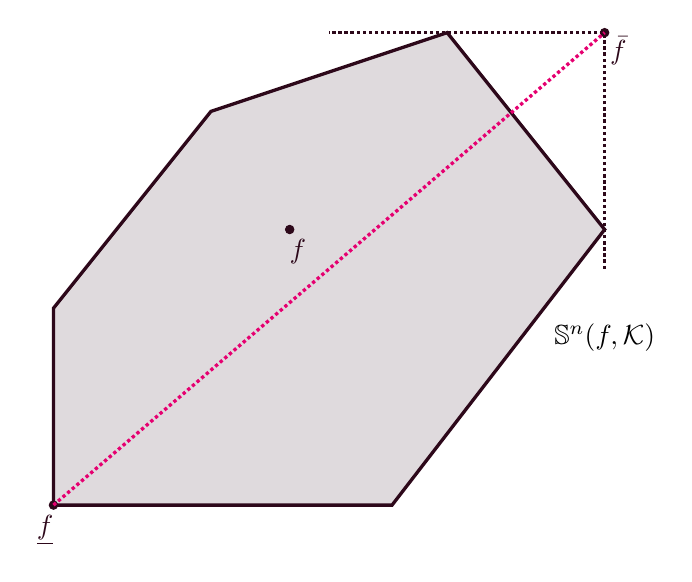
\begin{tikzpicture}[] %%[scale=4] ONLY changes distances, not the canvas
    % Define the coordinates of the vertices
    \coordinate (A) at (0, 0);
    \coordinate (B) at (4.3, 0);
    \coordinate (C) at (7, 3.5);
    \coordinate (D) at (5, 6);
    \coordinate (E) at (2, 5);
    \coordinate (F) at (0, 2.5);
    \coordinate (v) at (3, 3.5);
    \coordinate (vm) at (A);
    \coordinate (vM) at (7, 6);
    
    % Draw and fill the hexagon
		\filldraw[very thick, fill=white!85!mDarkBrown, draw=mDarkBrown] (A) -- (B) -- (C) node[anchor=north,yshift=-30]{$\mathbb{S}^n(f,\k)$}-- (D) -- (E) -- (F) -- cycle;

			    % \filldraw[mDarkBrown] (A) circle (1pt) node[anchor=north]{$A$};
			    % \filldraw[mDarkBrown] (B) circle (1pt) node[anchor=north]{$B$};
			    % \filldraw[mDarkBrown] (C) circle (1pt) node[anchor=west]{$C$};
			    % \filldraw[mDarkBrown] (D) circle (1pt) node[anchor=south]{$D$};
			    % \filldraw[mDarkBrown] (E) circle (1pt) node[anchor=south]{$E$};
			    % \filldraw[mDarkBrown] (F) circle (1pt) node[anchor=east]{$F$};

			    \filldraw[mDarkBrown] (v) circle (1.5pt) node[anchor=north,xshift=3]{${f}$};

			    \filldraw<2->[mDarkBrown] (vm) circle (1.5pt) node[anchor=north,xshift=-3]{${\underline f}$};
			    \filldraw<2->[mDarkBrown] (vM) circle (1.5pt) node[anchor=north,xshift=5,yshift=2]{${\bar f}$};
			    \draw<2->[densely dotted, very thick, draw=mDarkBrown] (7, 3) -- (vM) -- (3.5, 6);
			    \draw<3->[densely dotted, very thick, draw=mLightBrown] (vm) -- (vM);
		\end{tikzpicture}
	\end{center}
\end{frame}


\begin{frame}{Divergence}
	\begin{definition}[Divergence]
		Let $ f $ be a set function and $ \k \subseteq \k_0 $.
		Let $ \ell: \R^n \times \R^n \to \R^+_0 $.
		The \emph{divergence} is \[
			\fce{\Delta_\ell}{f, \k} \deq \fce{\ell}{\bar f_{\k}, \underline f_{\k}}.
		\]
	\end{definition}
	
	\vspace{2em}
	We only require $ \ell $ to satisfy the following: \[
		\left( \forall \k \supseteq \k_0 \right)\! \left( \forall S \subseteq N \right)\quad \fce{\Delta_\ell}{f, \k} \geq \fce{\Delta_\ell}{f, \k \cup S}.
	\]
\end{frame}

\begin{frame}{Reducing $ \Delta_\ell $ -- Setting}
	\begin{itemize}[ ]
		\item<2-> We have \alert<2>{$ f \sim \mathcal{F} $}, where $ \mathcal{F} $ is a distribution of superadditive set functions.
		\item<3-> We only \alert<3>{know $ \k \supseteq \k_0 $} values of it.
		\item<4-> We have a \alert<4>{budget $ \tau $} of how many values we can learn.
	\end{itemize}
\end{frame}

\begin{frame}{Reducing $ \Delta_\ell $ -- Offline Approach}
	In the simplest case, we can \alert{minimize the expected value}: \[
		\s^* = \argmin_{\s, \absolute{\s} = \tau} \E_{f \sim \mathcal{F}} \left[ \Delta_\ell(f,\k \cup \s) \right].
	\]

	\vspace{2em}
	We call this the \emph{Offline} approach.
\end{frame}

\begin{frame}{Reducing $ \Delta_\ell $ -- Online Approach}
	It is \textquote{inefficient} to learn all values at once.

	The \emph{Online} approach seeks to find a policy $ \pi $ which selects the next value to learn based on the values already known.

	A solution to the Online approach can be approximated using reinforcement learning (we use the PPO algorithm).
\end{frame}

\begin{frame}{Reducing $ \Delta_\ell $ -- Results for $ \mathcal{F} = \texttt{factory} (5) $}
	\begin{center}
		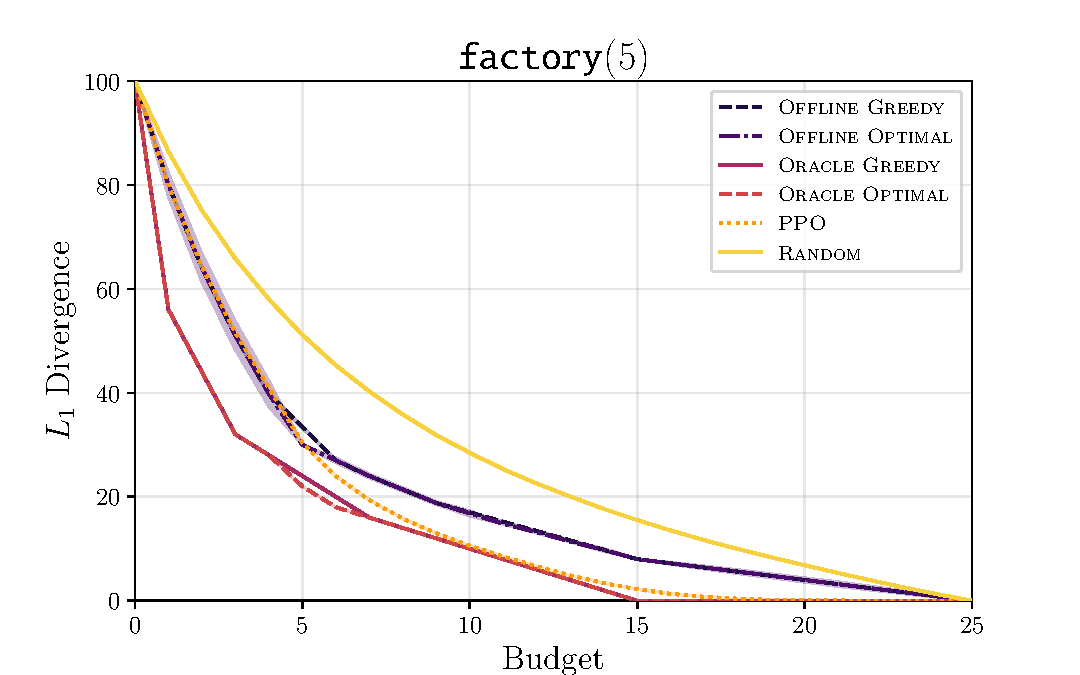
\includegraphics[width=.8\textwidth]{figures/l1_norm_predictible_factory5.pdf}
	\end{center}
\end{frame}

\begin{frame}{Supermodular Functions}
	\begin{definition}[Supermodular Function]
		A set function $ f $ is \emph{supermodular} $ \equiv $ \[
			\left( \forall S,T \subseteq N \right)\quad \fce{f}{S} + \fce{f}{T} \leq \fce{f}{S \cup T} + \fce{f}{S \cap T}.
		\]
	\end{definition}
	
\end{frame}

\begin{frame}{Reducing $ \Delta_\ell $ -- Results for $ \mathcal{F} = \texttt{supermodular} (5) $}
	\begin{center}
		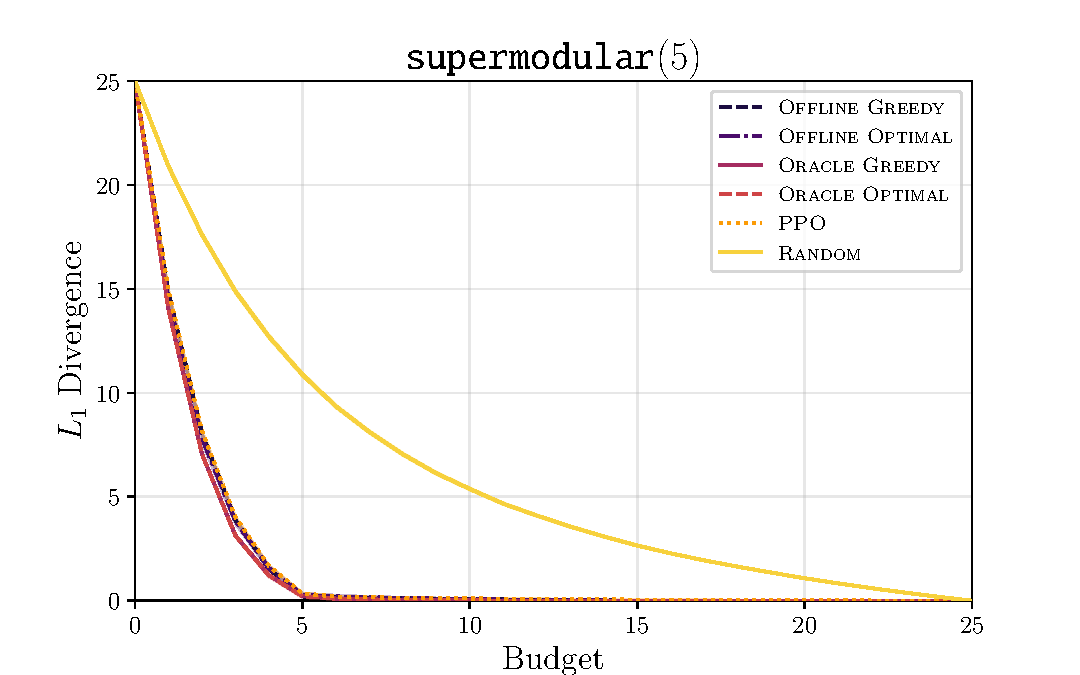
\includegraphics[width=.8\textwidth]{figures/l1_norm_convex5.pdf}
	\end{center}
\end{frame}

\begin{frame}{Reducing $ \Delta_\ell $ -- \textsc{Largest Subsets} Heuristic}
	\begin{center}
		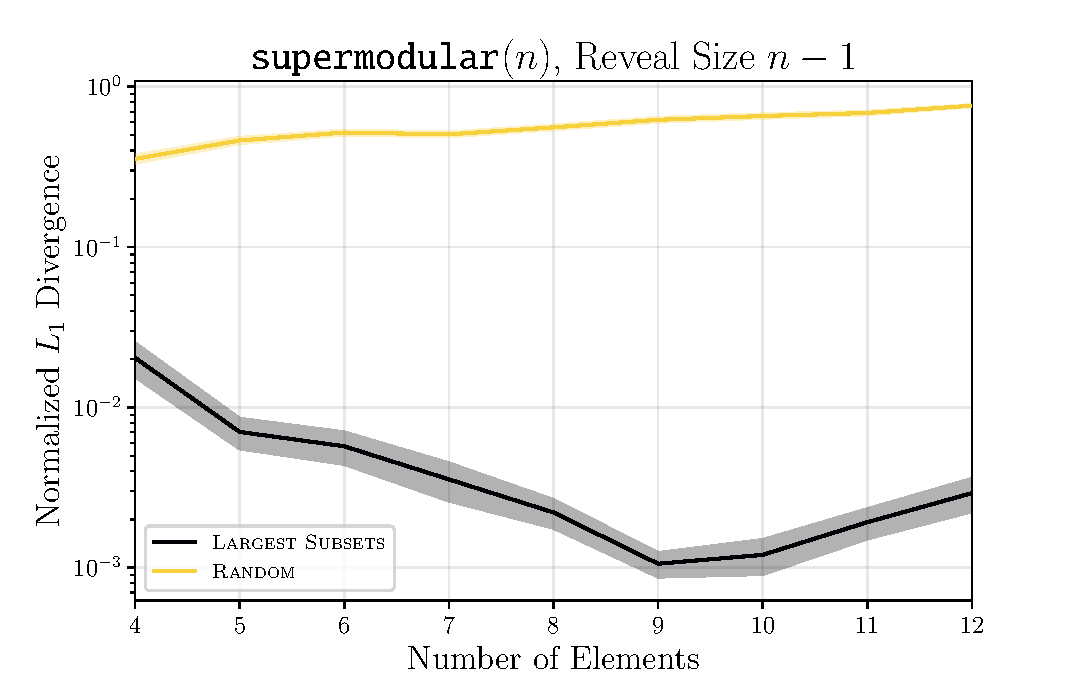
\includegraphics[width=.8\textwidth]{figures/l1_norm_convex_linear.pdf}
	\end{center}
\end{frame}

\begin{frame}{Conclusion}
	\begin{itemize}
		\item Set functions grow exponentially with the size of $ N $.
		\item We limit their size to $ \k \subseteq \pot N $ subsets.
		\item We propose a way to quantify the resulting ambiguity.
		\item We investigate how to choose $ \k $, such that the ambiguity is minimised.
		\item We explore both Offline and Online approaches to this problem.
	\end{itemize}
\end{frame}

\appendix

\begin{frame}{}
	\begin{quote}
		Definice nosiče na str. 4 je vágní, není jasné, co se myslí “the set of values it can have.” Nosič náhodné veličiny se definuje jako nosič její pravděpodobnostní distribuce a nehrozí tak záměna různých pojmů nosiče (např. v matematické analýze je nosičem funkce uzávěr množiny nenulových hodnot té funkce).
	\end{quote}
	
	 
\end{frame}

\begin{frame}
	\begin{quote}
		“The formed coalitions receive some value.” Raději worth místo “value”.
	\end{quote}
\end{frame}

\begin{frame}
	\begin{quote}
		Figure 1.1. V argumentech funkce $ \tau $ chybí $ a_t $.
	\end{quote}
	\begin{center}
		\vspace{2em}
		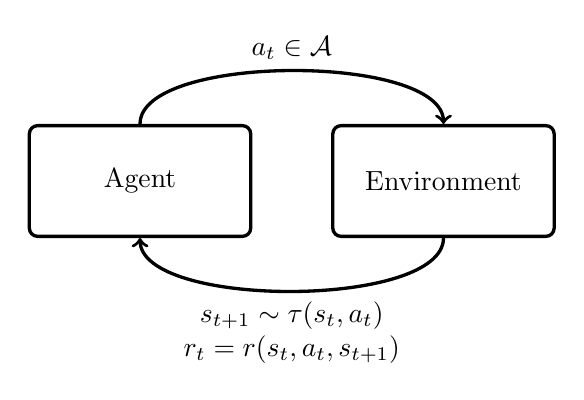
\begin{tikzpicture}[
		stff/.style={rectangle, draw=black, very thick, minimum height=40, minimum width=80, rounded corners=3},
		]
			%Nodes
			\node[stff]        (Agent)                            {Agent};
			\node[stff]        (Environment)   [right=of Agent]   {Environment};

			%Lines
			\draw[->, very thick] (Agent.north)  .. controls  +(up:9mm) and +(up:9mm) .. node[midway, above] {$ a_t \in \mathcal{A} $} (Environment.north);
			\draw[->, very thick] (Environment.south)  .. controls  +(up:-9mm) and +(up:-9mm) .. node[midway, below, align=center] {$ s_{t+1} \sim \fce{\tau}{s_{t}, \alert{a_t}} $\\$ r_t = \fce{r}{s_{t}, a_t, s_{t+1}} $} (Agent.south);
		\end{tikzpicture}
	\end{center}
\end{frame}

\begin{frame}
	\begin{quote}
		Pojmy “MDP” a “environment” se užívají jako synonyma (Definice 10 a Definice 11). To je v pořádku, jen by si to zasloužilo krátký komentář.
	\end{quote}
\end{frame}

\begin{frame}
	\begin{quote}
		Notace $ \E_\pi [G_0] $ se liší od notace pro střední hodnotu v Definici 13 a o 3 řádky dále je v textu použita ještě jiná notace.
	\end{quote}

When constructing a policy, our goal is to maximize $ \fceb{\E}{G_0} $, where the expectation is taken over the initial state, the transition function, and the policy in each step.
It is sometimes useful to explicitly state the policy used by the agent in the notation.
For that, we use the notation $ \fceb{\E_\pi}{G_0} $, which is common in RL literature, signaling that the actions chosen when computing the return are corresponding to the policy $ \pi $.

\hfill -- Strana 9

\end{frame}

\begin{frame}
	\begin{quote}
		Na str. 13 “a player may claim he is more valuable to the grand coalition” není nutně pravda, protože hodnota hráče je určena jeho příspěvkem ke všem možným koalicím.
	\end{quote}
\end{frame}

\begin{frame}
	\begin{quote}
		Definice 15. “Incomplete set function” je restrikcí funkce $ f $ na $ \k $. Možná by se dala použít pro restrikci notace $ f_\k $, což formálně podtrhuje nutnost pracovat s $ f $ i s její restrikcí.
	\end{quote}

	\vspace{2em}
	\begin{definition}[Incomplete set function]
		Let $ f: \pot N \to \R $ be a set function.
		An \emph{incomplete set function} is $ \left( f, \k \right) $, where $ \k \subseteq \pot N $ are the subsets with \emph{known values} of the set function.
	\end{definition}
\end{frame}

\begin{frame}
	\begin{quote}
		Stavový prostor policy $ \pi $ na str. 19 (druhý odstavec) má být $ \pot{\pot \N \times \R} \times \N $.
	\end{quote}
	\vspace{2em}
	Notice that the policy used here matches the definition of a policy we have given as Definition 11 in Section 1.3, with $ \pot {\alert{\pot N} \times \R} \times \N $ as the state space, and $ \pot N \setminus \k_0 $ as the action space.
\end{frame}

\end{document}
